% Downloaded MB
\begin{figure*}[th]
    \centering
    \subfloat[\textbf{Pre-lockdown weekdays.} Average volume of downloaded data per test unit, broken down by the hour of the day, on weekdays in the pre-lockdown time period. \label{download-a}]{%
      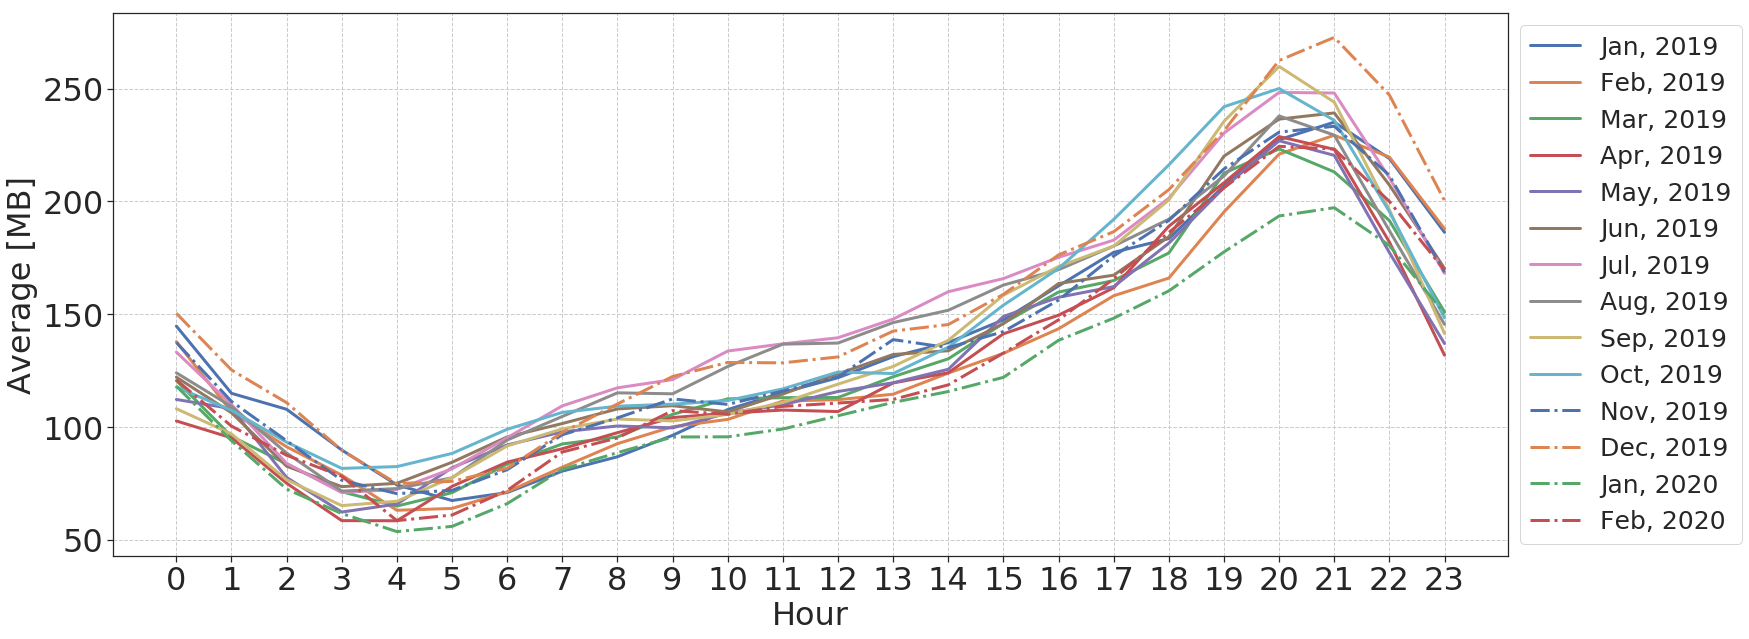
\includegraphics[width=0.48\linewidth]{figs/wenjun/download_wdays_before.png}%
    }
    \hfil
    \subfloat[\textbf{Pre-lockdown weekends.} Average volume of downloaded data per test unit, broken down by the hour of the day, on weekends in the pre-lockdown time period. \label{download-b}]{%
        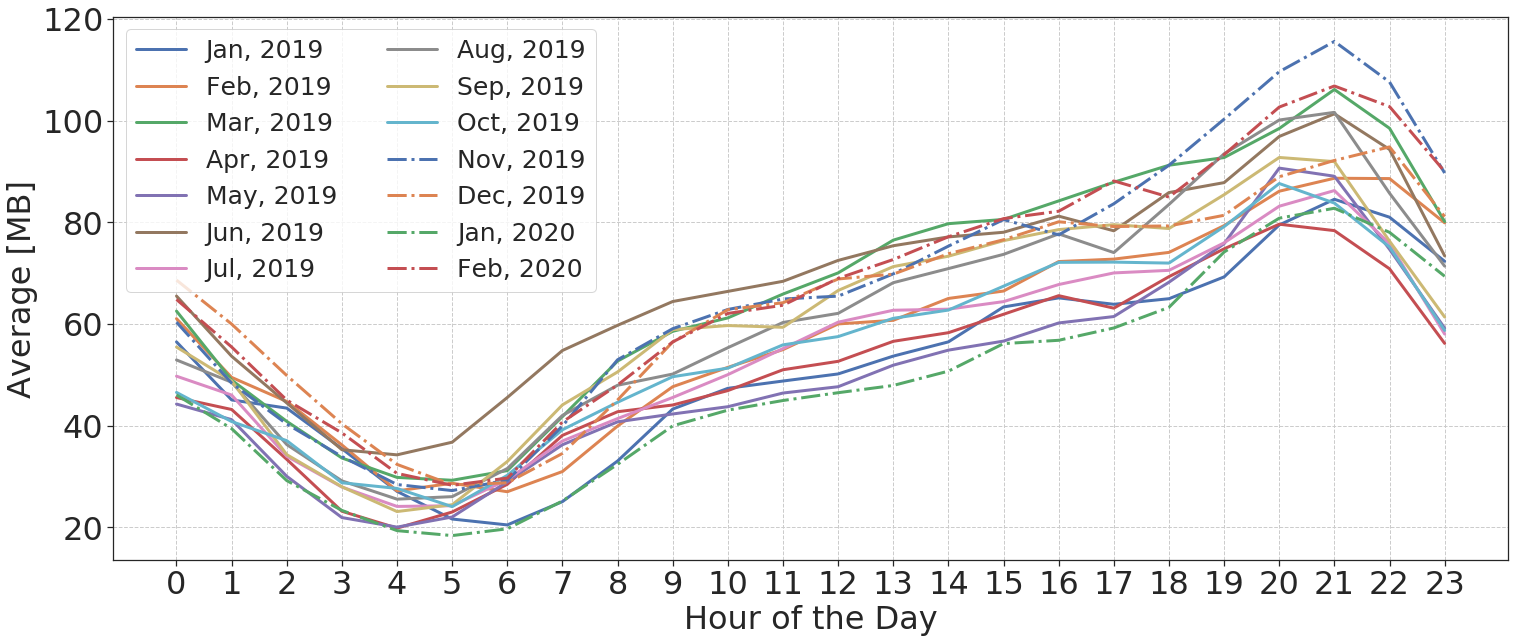
\includegraphics[width=0.48\linewidth]{figs/wenjun/download_wends_before.png}%
    }
    \\
    \subfloat[\textbf{Lockdown weekdays.} Average volume of downloaded data per test unit, broken down by the hour of the day, on weekdays in the lockdown time period. \label{download-c}]{%
        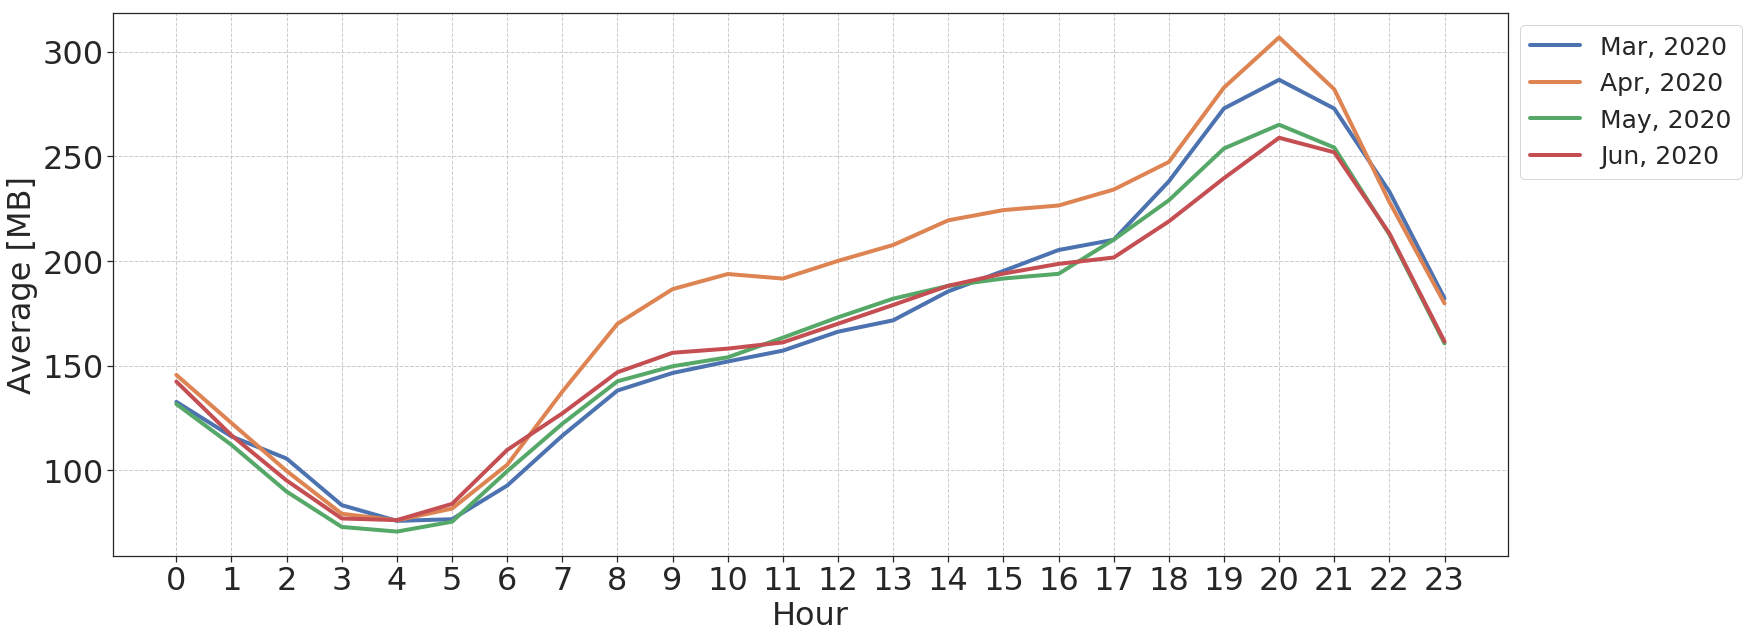
\includegraphics[width=0.48\linewidth]{figs/wenjun/download_wdays_after.png}%
    }
    \hfil
    \subfloat[\textbf{Lockdown weekends.} Average volume of downloaded data per test unit, broken down by the hour of the day, on weekends in the lockdown time period. \label{download-d}]{%
        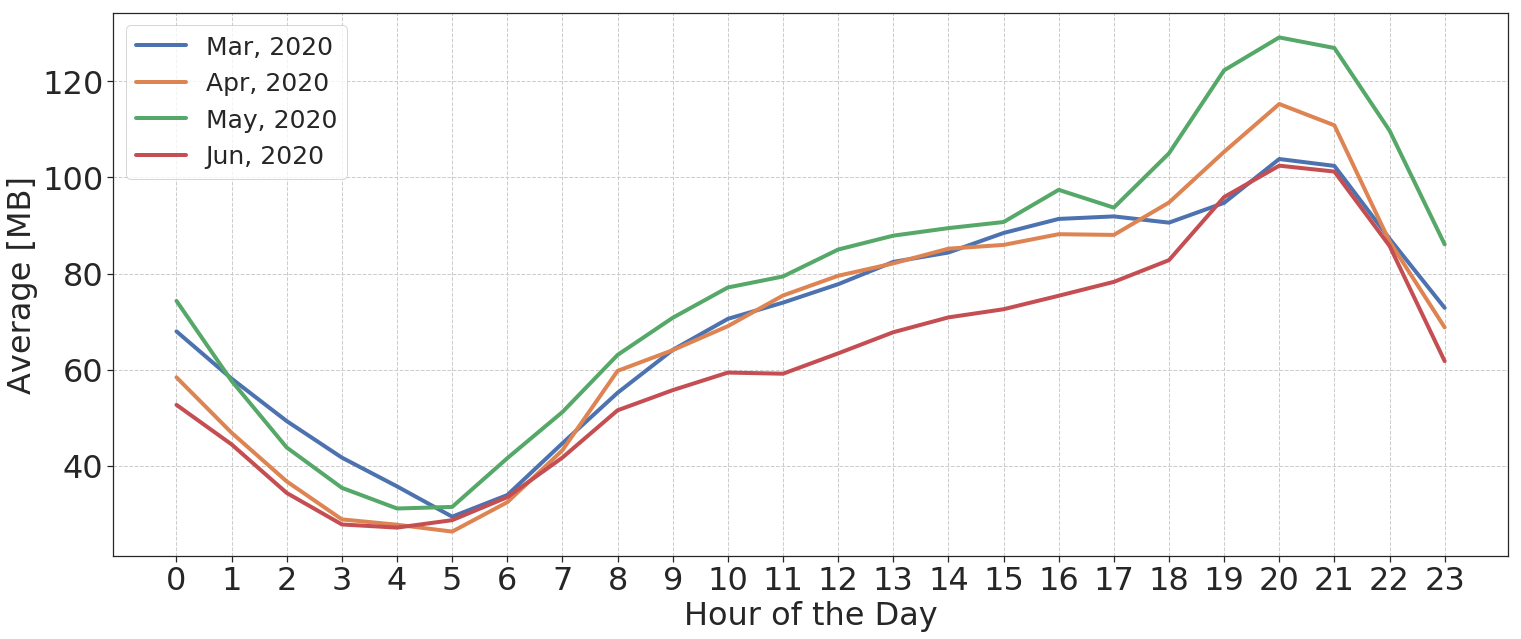
\includegraphics[width=0.48\linewidth]{figs/wenjun/download_wends_after.png}%
    }
    \\
    \subfloat[\textbf{2019 vs 2020 weekdays.} Average volume of downloaded data per test unit on weekdays in March-June compared between 2019 and 2020.
    \label{download-e}]{%
        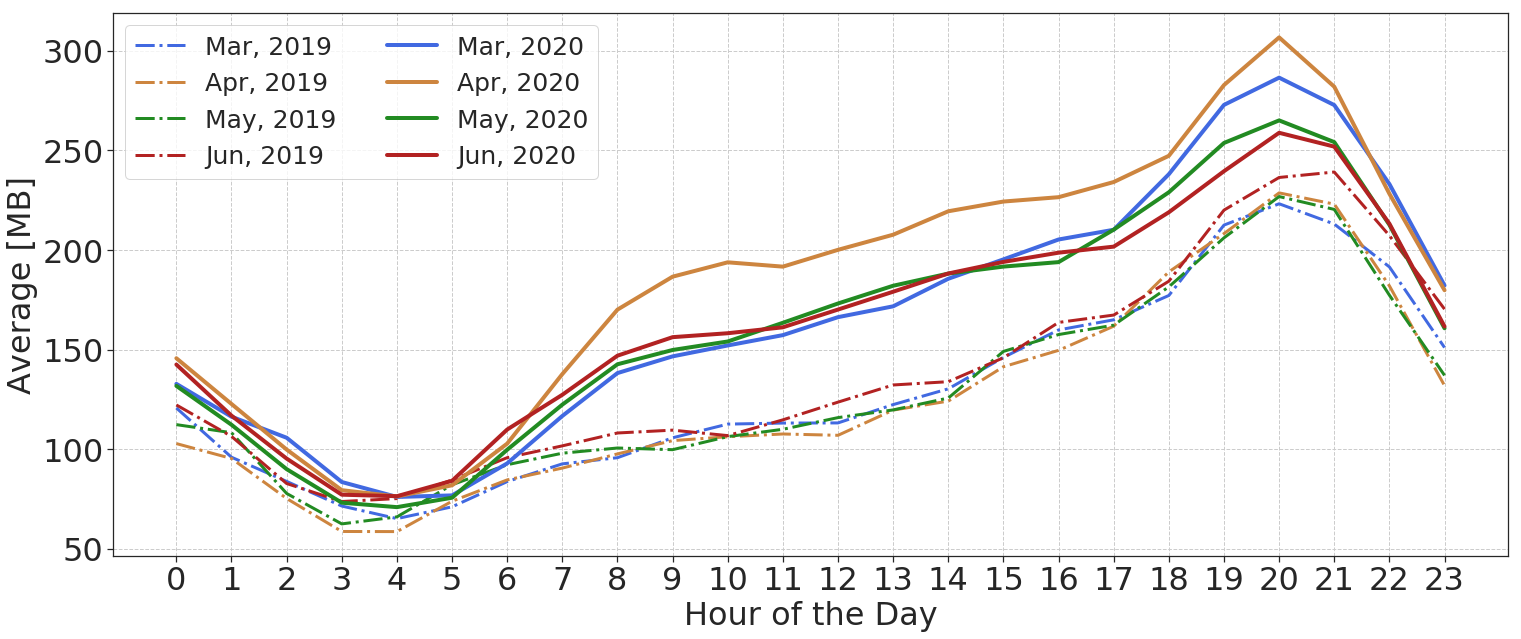
\includegraphics[width=0.48\linewidth]{figs/wenjun/download_wdays_compare_36.png}%
    }
    \hfil
    \subfloat[\textbf{2019 vs 2020 weekends.} Average volume of downloaded data per test unit on weekends in March-June compared between 2019 and 2020.
    \label{download-f}]{%
        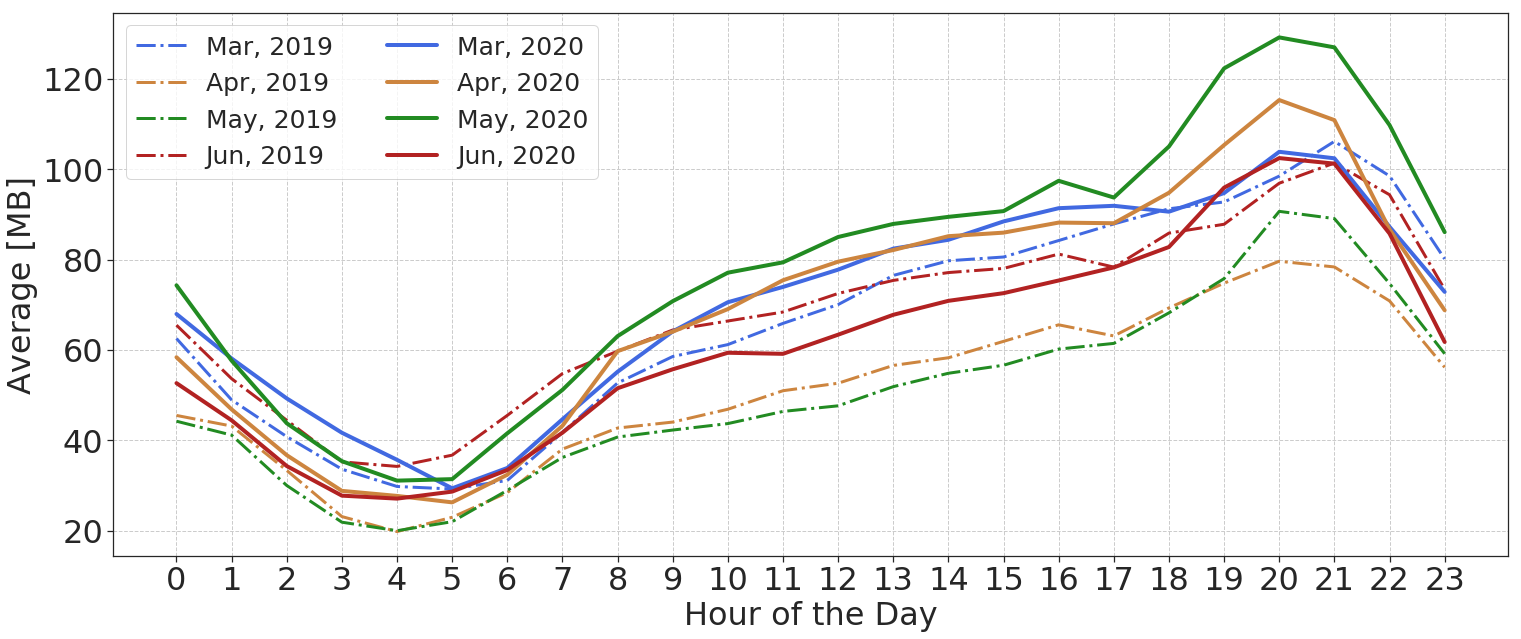
\includegraphics[width=0.48\linewidth]{figs/wenjun/download_wends_compare_36.png}%
    }

    \caption{Graphs comparing and contrasting the average hourly downloaded volume of data per test unit in various time periods. The peak is always between 18:00 and 22:00, which is the internet rush hour. The volumes in the lockdown time period are generally larger than the volumes in the pre-lockdown time period. Lockdown weekday traffic patterns start to resemble weekend patterns.}
    \label{fig:download-data-per-user-hours-fig}
\end{figure*}

\begin{figure*}[th]
    \centering
    \subfloat[\textbf{Pre-lockdown weekdays.} Average volume of uploaded data per test unit, broken down by the hour of the day, on weekdays in the pre-lockdown time period.
    \label{upload-a}]{%
        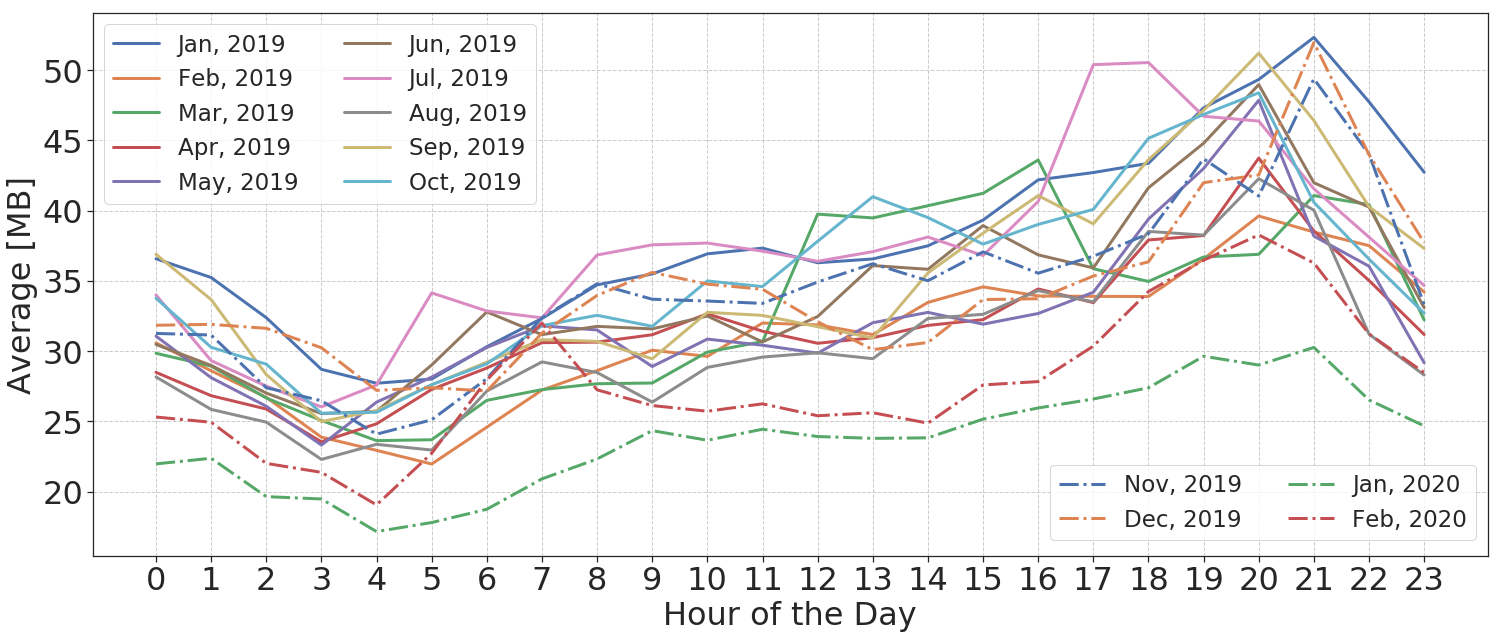
\includegraphics[width=0.48\linewidth]{figs/wenjun/upload_wdays_before.png}%
    }
    \hfil
    \subfloat[\textbf{Pre-lockdown weekends.} Average volume of uploaded data per test unit, broken down by the hour of the day, on weekends in the pre-lockdown time period.
    \label{upload-b}]{%
        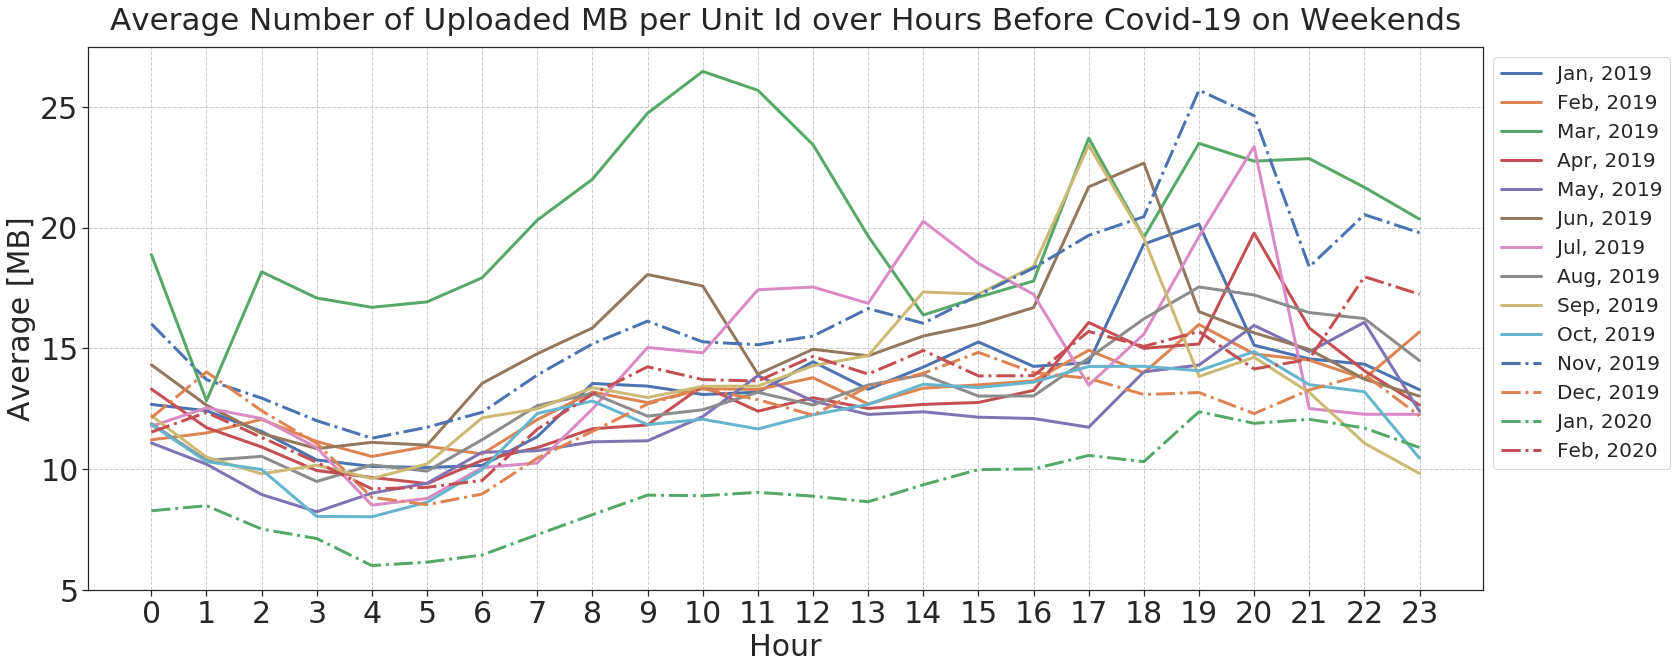
\includegraphics[width=0.48\linewidth]{figs/wenjun/upload_wends_before.png}%
    }
    \\
    \subfloat[\textbf{Lockdown weekdays.} Average volume of uploaded data per test unit, broken down by the hour of the day, on weekdays in the lockdown time period.
    \label{upload-c}]{%
        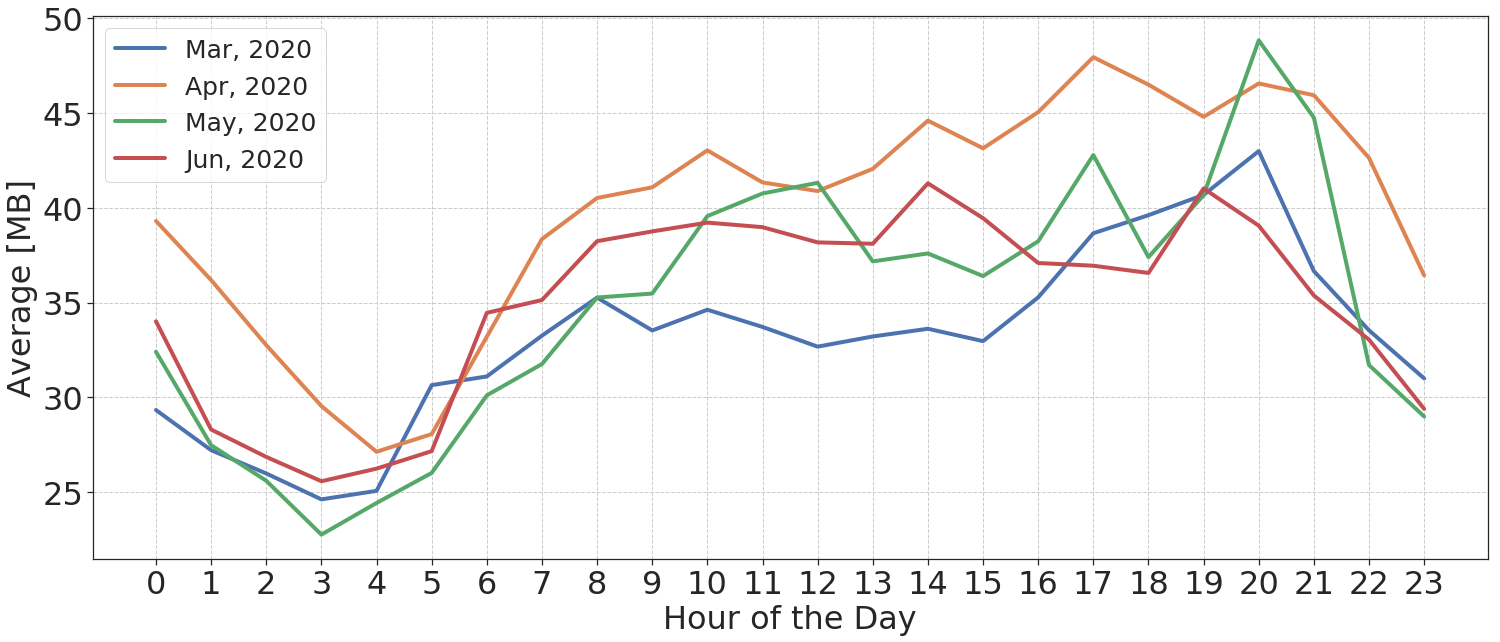
\includegraphics[width=0.48\linewidth]{figs/wenjun/upload_wdays_after.png}%
    }
    \hfil
    \subfloat[\textbf{Lockdown weekends.} Average volume of uploaded data per test unit, broken down by the hour of the day, on weekends in the lockdown time period. \label{upload-d}]{%
        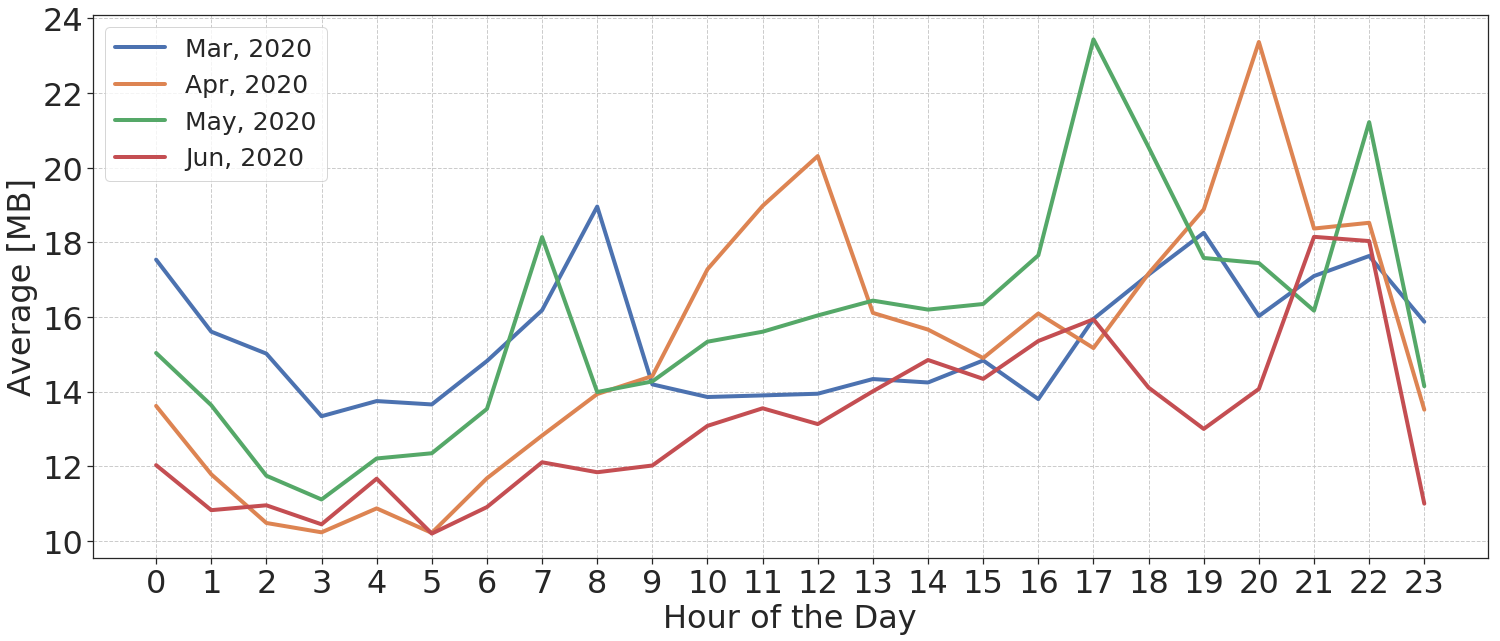
\includegraphics[width=0.48\linewidth]{figs/wenjun/upload_wends_after.png}%
    }
    \\
    \subfloat[\textbf{2019 vs 2020 weekdays.} Average volume of uploaded data per test unit on weekdays in March-June compared between 2019 and 2020.
    \label{upload-e}]{%
        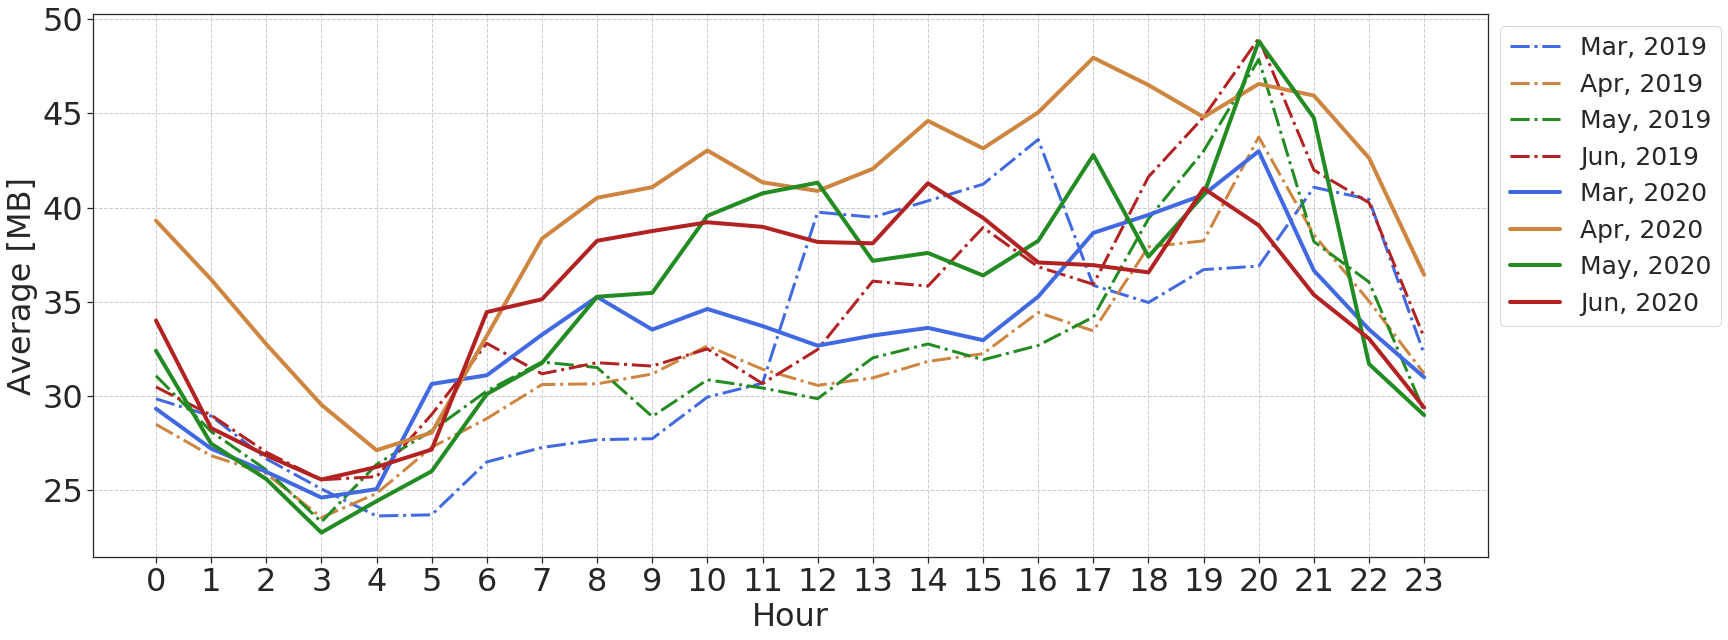
\includegraphics[width=0.48\linewidth]{figs/wenjun/upload_wdays_compare_36.png}%
    }
    \hfil
    \subfloat[\textbf{2019 vs 2020 weekends.} Average volume of uploaded data per test unit on weekends in March-June compared between 2019 and 2020.
    \label{upload-f}]{%
        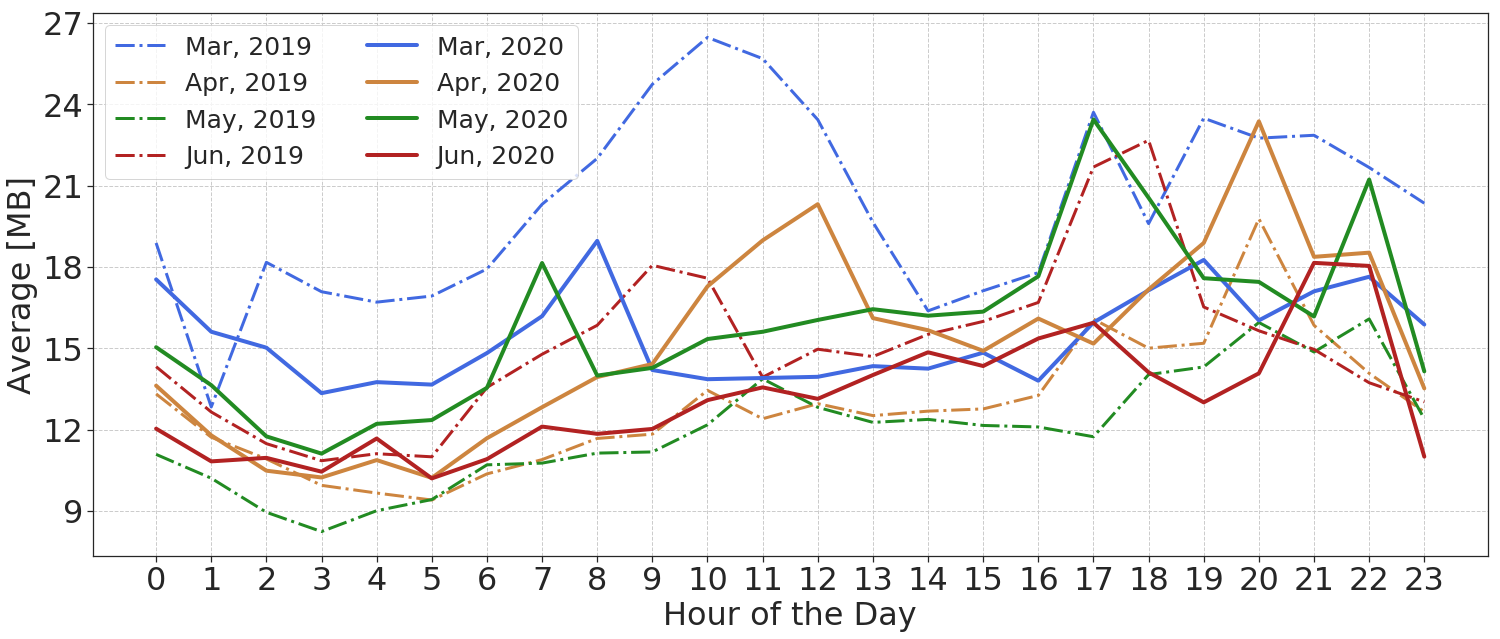
\includegraphics[width=0.48\linewidth]{figs/wenjun/upload_wends_compare_36.png}%
    }

    \caption{Graphs comparing and contrasting the average hourly upload volume of data per test unit in various time periods. Compared with download patterns, the lines in these graphs fluctuate more, especially on weekends. When comparing April and May between 2019 and 2020, we see an overall increase in uploaded data in 2020.}
  \label{fig:upload_data_per_user_hours_fig}
\end{figure*}


\section{Hourly Data Usage Patterns}
\label{sec:hourly-data-usage-patterns}

Hourly data usage patterns (upload and download) could potentially provide insights into the behavior of fixed broadband internet users before and during the pandemic. Some applications such as music and video streaming generally increase the volume of downloaded data. Other applications such as VoIP, video conferencing, or networked games influence the volume of uploaded data.

In this section, we study the average hourly data usage per test unit from multiple perspectives and attempt to correlate the observations with changing user behavior patterns during the lockdown. We contrast weekday and weekend patterns, analyze the differences in uploaded and downloaded traffic volumes, and compare with the data from the corresponding period of 2019 to eliminate potential seasonal differences.

The analysis in this section is primarily based on the ``datausage'' table from the FCC MBA raw dataset. That table keeps track of the total number of bytes received and transmitted by all user's devices within each hour of the day. For hourly analysis, we needed to translate UTC timestamps to the test unit's local time using the unit profile dataset, as described in Section \ref{sec:methodology}. All graphs in this section were generated with measurements from approximately 3000 test units.

\subsection{Analysis of Download Patterns}
\label{sec:analysis-of-download-patterns}

% internet rush hour explanation
All graphs in \figurename~\ref{fig:download-data-per-user-hours-fig} show a traffic peak between 18:00 and 22:00 hours, also known as the internet rush hour \cite{internetrushhour}. Most likely explanation for this peak is post-workday internet multi-media consumption for entertainment purposes, e.g., Netflix or Youtube.

% pre-lockdown weekday versus weekend
Graphs in \figurename~\ref{download-a} and \ref{download-b} compare average weekday and weekend download traffic volumes in the pre-lockdown period, i.e., until end of February 2020. We clearly see that the overall average download volume is higher on weekdays. However, the distribution of activity throughout the day is different for weekdays and weekends. Between approximately 9:00 and 17:00, the weekend graph shows a relative increase in traffic volumes compared to the weekday graph and more variability month-to-month. This corresponds with the intuition that users typically use fixed broadband internet more during weekends when they are at home. The increase in variability can probably be partially explained by seasonal effects.

% pre-lockdown weekend versus lockdown weekend
\figurename~\ref{download-b} and \ref{download-d} compare weekend traffic before and during lockdown. We see that the minimum and maximum weekend daily traffic levels are roughly the same before and during lockdown. In March--May 2020 we see a significant increase in daytime weekend traffic volumes (green, yellow, blue in \figurename~\ref{download-d}) relative to the period before lockdown. Interestingly, daytime volumes return to their normal pre-lockdown levels in June 2020. This can be partially explained by the fact that many restrictions in effect since April were being relaxed by June. As a result, some users may have returned to spending their weekends outside of the home. % Maybe mention that this is consistent with "new normal" in one of the papers in Related Work.

% lockdown weekday versus weekend
When we compare lockdown weekdays with weekends in \figurename~\ref{download-c} and \ref{download-d}, we see that the hourly weekday pattern starts to resemble weekend patterns. This trend is particularly visible for April 2020 (yellow). This trend is also clearly visible in \figurename~\ref{download-e} which contrasts lockdown weekday data with weekday data from the same period of 2019. We clearly see that 2019 and 2020 curves cluster in two separate regions during daytime from roughly 8:00 to 18:00 hours. In other words, lockdown weekday download patterns morphed into weekend patterns. The same trend was observed by other authors in data from different vantage points.% Cite a specific paper.

% lockdown weekday detail
It is worth nothing that in \figurename~\ref{download-c} April 2020 appears to be an outlier. All other lockdown months appear to converge to similar traffic levels. Somewhat lower traffic levels in May and June 2020 can be probably partially explained by: a) a new normal, b) relaxed lockdown restrictions. The traffic levels are highest in April because it is the first month in which most of the US states were under a mandatory lockdown. Thus, this month represents the initial lockdown period during which a significant proportion of users was getting accustomed to working from home or online learning activities. The increase in evening traffic levels is likely due to social distancing restrictions \cite{lockdownsguide}, where people moved social activities to the internet.

% lockdown weekend detail
On weekends (\figurename~\ref{download-f}), we see a small traffic increase in March, and the increases in April and May are substantial. Weekend June 2020 daytime traffic levels saw a relative decrease compared with June 2019 levels, except for the evening spike. One way to explain the difference might be that after months of restrictions people try to spend weekends more outside their homes. This pattern coincides with the policies related to COVID-19 in the United States: the height of restriction was at the end of March and the beginning of April, and some restrictions were being relaxed in the mid-late May or June in many states \cite{covid19restriction}.

We conclude that people use fixed broadband internet more and download more data because of COVID-19 and its related policies (e.g., lockdown, quarantine, work from home, etc.).

\subsection{Analysis of Upload Patterns}
\label{sec:analysis-of-upload-patterns}

\figurename~\ref{fig:upload_data_per_user_hours_fig} shows several plots of hourly average uploaded data. As expected, there is significantly more noise and fluctuation in these plots (particularly weekends), compared with the download plots in \figurename~\ref{fig:download-data-per-user-hours-fig}.

We note that we have no explanation for the morning spike in March 2019 shown in \figurename~\ref{upload-b}. Unlike the corresponding download patterns, hourly upload patterns before lockdown show little difference between weekdays and weekends, partly due to the noise.

 The average uploaded data levels April and May 2020 are larger than those in 2019, but in March and June, that is not the case (\figurename~\ref{upload-e} and \ref{upload-f}). Possible reasons might be similar to those discussed earlier: the majority of US states enforced peak lockdown restrictions at the end of March and the beginning of April. Some of the restrictions ended in mid-late May or June in some states \cite{covid19restriction}.

 On weekdays, the daytime average uploaded data levels in April, May, and June 2020 are much larger than those in the corresponding months of 2019. On weekends, the increase is relatively smaller than on weekdays.